\documentclass[../main.tex]{subfiles}

\subsection{Interferenz}
\begin{frame}
    \frametitle{Grundlagen}
    \framesubtitle{Interferenz}
    \begin{columns}
        \column{0.5\textwidth}
        \begin{block}{Konstruktive Interferenz}
            $\Delta s = m \cdot \lambda$
        \end{block}
        \begin{block}{Destruktive Interferenz}
            $\Delta s = \lambda \cdot m - \lambda \cdot \frac{1}{2}$
        \end{block}
        \begin{alertblock}{Summenformel}
            $f_{ges}(x_0, t) = \sum_{i}f_i(x_0, t)$
        \end{alertblock}
        \column{0.5\textwidth}
        \begin{figure}
            \begin{tikzpicture}
            \begin{axis}[
                xmin=0,xmax=31.4,
                ymin=-3,ymax=3,
                ticks=none,
                axis line style=white,
                scale only axis,
                domain=0:31.4,
                height=0.2\textheight
            ]
                \addplot[gray,dashed,thin]{2};
                \addplot[samples=200,blue] {sin(deg(x))/2+2};
                \addplot[gray,dashed,thin]{0};
                \addplot[samples=200,blue] {sin(deg(x))/2};
                \addplot[gray,dashed,thin]{-2};
                \addplot[samples=200,blue,very thick] {sin(deg(x))-2};
            \end{axis}
            \end{tikzpicture}
        \end{figure}
        \begin{figure}
            \begin{tikzpicture}
            \begin{axis}[
                xmin=0,xmax=31.4,
                ymin=-3,ymax=3,
                ticks=none,
                axis line style=white,
                scale only axis,
                domain=0:31.4,
                height=0.2\textheight
            ]
                \addplot[gray,dashed,thin]{2};
                \addplot[samples=200,blue] {sin(deg(x+3.14))/2+2};
                \addplot[gray,dashed,thin]{0};
                \addplot[samples=200,blue] {sin(deg(x))/2};
                \addplot[gray,dashed,thin]{-2};
                \addplot[samples=200,blue,very thick] {-2};
            \end{axis}
            \end{tikzpicture}
        \end{figure}
    \end{columns}
\end{frame}

\subsection{Doppelspaltexperiment}
\begin{frame}
    \frametitle{Grundlagen}
    \framesubtitle{Doppelspaltexperiment}
    \begin{columns}
        \column{0.4\textwidth}
        \begin{itemize}
            \item Parallelwellen $\rightarrow$ Elementarwellen
            \item Interferenzmuster
            \begin{itemize}
                \item Maxima: Konstruktive I.
                \item Minima: Destruktive I.
            \end{itemize}
        \end{itemize}
        \column{0.6\textwidth}
        \begin{figure}[ht]
            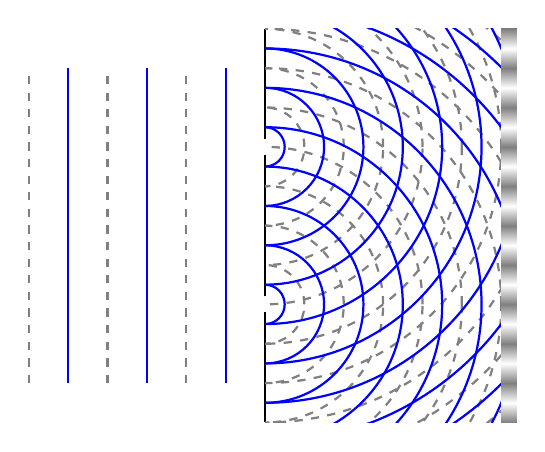
\begin{tikzpicture}
                % Parallel Waves
                \foreach \i in {0.5,1.5,...,2.5}
                    \draw[blue,thick] ({\i},2) -- ({\i},6); % Hochpunkte

                \foreach \i in {0,1,...,2.5}
                    \draw[gray,dashed,thick] ({\i},2) -- ({\i},6); % Tiefpunkte
                
                % Double Slit @ 3 & 5
                \draw[thick] (3,1.5) -- (3,2.9);
                \draw[thick] (3,3.1) -- (3,4.9);
                \draw[thick] (3,5.1) -- (3,6.5);
                
                % Elementary waves
                \begin{scope}
                    \clip (3,1.5) rectangle (6,6.5);
                    
                    \foreach \i in {0.5,1,...,5} { % Tiefpunkte
                        \draw[gray, dashed,thick] (3,5) circle(\i);
                        \draw[gray, dashed,thick] (3,3) circle(\i);
                    }
                    \foreach \i in {0.25,0.75,...,5} { % Hochpunkte
                        \draw[blue,thick] (3,5) circle(\i);
                        \draw[blue,thick] (3,3) circle(\i);
                    }
                \end{scope}

                % Interference pattern
                \foreach \i in {1,2,...,20}
                    \shade[black,white,shading angle={mod(\i,20)*180}] (6,{\i/4+1.25}) rectangle (6.2,{\i/4+1.5});
            \end{tikzpicture}
        \end{figure}
    \end{columns}
\end{frame}

\subsection{Absorption}
\begin{frame}
    \frametitle{Grundlagen}
    \framesubtitle{Absorption}

    \begin{columns}
        \column{0.5\textwidth}
        \begin{block}{}
            Aufnahme von Wellen in einer Substanz
        \end{block}
        \begin{itemize}
            \item Absorption in Form von Vibration
        \end{itemize}
        \column{0.5\textwidth}
        % Absorption
        \begin{figure}
            \begin{tikzpicture}
                \draw[white] (0,0) grid (2,2);
                \draw[very thick,blue] (0.5,1) -- (1.5,1);
                \draw (1,2) -- (1,1);
                \draw[->,dashed] (1,1) -- (1,0);
            \end{tikzpicture}
        \end{figure}
    \end{columns}
\begin{figure}[ht]
        \centering
        \begin{subfigure}[b]{0.3\textwidth}
            \resizebox{\textwidth}{!} {
                \chemfig{
                    O(-[:135,0.8]H)(-[:45,0.8]H)
                }
                \hspace{0.1cm}
                \chemfig{
                    O(-[:135,1.2]H)(-[:45,1.2]H)
                }
            }
            \caption{\SI{2.8}{\micro\metre}}
        \end{subfigure}
        \vrule
        \begin{subfigure}[b]{0.3\textwidth}
            \resizebox{\textwidth}{!} {
                \chemfig{
                    O(-[:135]H)(-[:45]H)
                }
                \hspace{0.1cm}
                \chemfig{
                    O(-[:160]H)(-[:20]H)
                }
            }
            \caption{\SI{5.3}{\micro\metre}}
        \end{subfigure}
        \vrule
        \begin{subfigure}[b]{0.3\textwidth}
            \resizebox{\textwidth}{!} {
                \chemfig{
                    O(-[:135,1.2]H)(-[:45,0.8]H)
                }
                \hspace{0.1cm}
                \chemfig{
                    O(-[:135,0.8]H)(-[:45,1.2]H)
                }
            }
            \caption{\SI{2.8}{\micro\metre}}
        \end{subfigure}
        \caption{Vibrationsmuster des $H_2O$-Moleküls}
    \end{figure}
\end{frame}

\begin{frame}
    \frametitle{Grundlagen}
    \framesubtitle{Absorption}

    \begin{figure}[ht]
        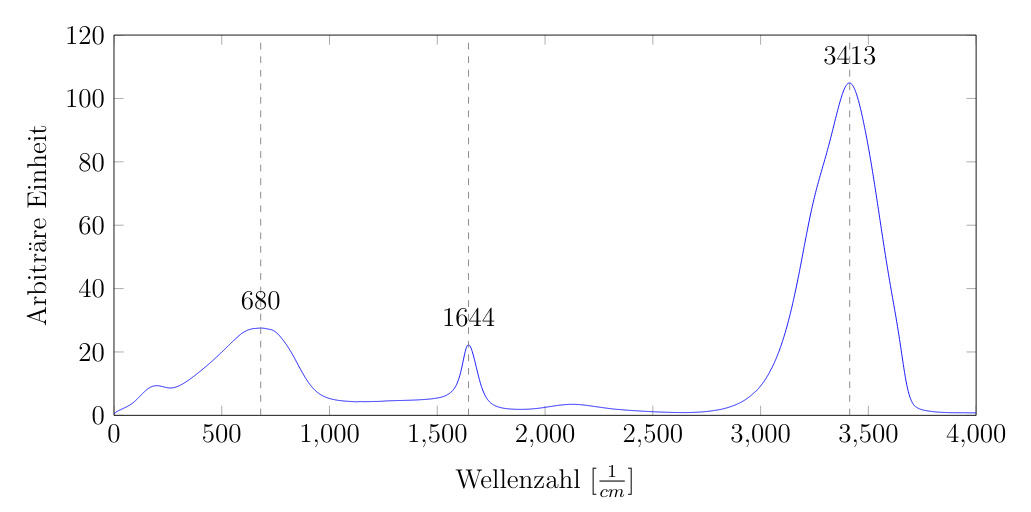
\includegraphics[width=\textwidth,height=\textheight,keepaspectratio]{assets/images/wasser_diagramm.png}
        \caption{Molarer Absorptionsgrad von $H_2O$ bei \SI{25}{\celsius}}
    \end{figure}
\end{frame}